%%%%%%%%%%%%%%%%%%%%%%%%%%%%%%%%%%%%%%%%%%%%%%%%%%%
%
%  New template code for TAMU Theses and Dissertations starting Fall 2012.  
%  For more info about this template or the 
%  TAMU LaTeX User's Group, see http://www.howdy.me/.
%
%  Author: Wendy Lynn Turner 
%	 Version 1.0 
%  Last updated 8/5/2012
%
%%%%%%%%%%%%%%%%%%%%%%%%%%%%%%%%%%%%%%%%%%%%%%%%%%%
%%%                           SECTION II
%%%%%%%%%%%%%%%%%%%%%%%%%%%%%%%%%%%%%%%%%%%%%%%%%%%
\chapter{\uppercase {The DFEM Formulation of the Multigroup $S_N$ Equations}}
\label{sec::Sn}

The movement of bulk materials and particles through some medium can be described with the statistical behavior of a non-equilibrium system. Boltzmann first devised these probabilistic field equations to characterize fluid flow via driving temperature gradients \cite{encyc_physics}. His work was later extended to model general fluid flow, heat conduction, hamiltonian mechanics, quantum theory, general relativity, and radiation transport, among others. The Boltzmann Equation can be written in the general form:

\begin{equation}
\label{eq::gen_boltzmann}
\frac{\partial u}{\partial t} = \left( \frac{\partial u}{\partial t}  \right)_{force} + \left( \frac{\partial u}{\partial t}  \right)_{advec} + \left( \frac{\partial u}{\partial t}  \right)_{coll}
\end{equation}

\noindent where $u(\vec{r},\vec{p},t)$ is the transport distribution function parameterized in terms of position, $\vec{r}=(x,y,z)$, momentum, $\vec{p}=(p_x,p_y,p_z)$, and time, $t$. In simplified terms, Eq. (\ref{eq::gen_boltzmann}) can be interpreted that the time rate of the change of the distribution function, $\frac{\partial u}{\partial t}$, is equal to the sum of the change rates due to external forces, $\left( \frac{\partial u}{\partial t}  \right)_{force} $, advection of the particles, $\left( \frac{\partial u}{\partial t}  \right)_{advec}$, and particle-to-particle and particle-to-matter collisions, $\left( \frac{\partial u}{\partial t}  \right)_{coll}$ \cite{mcgraw_physics}. 

For neutral particle transport, the following assumptions \cite{duderstadt1979transport} about the behavior of the radiation particles can be utilized:

\begin{enumerate}
	\item Particles may be considered as points;
	\item Particles do not interact with other particles;
	\item Particles interact with material target atoms in a binary manner;
	\item Collisions between particles and material target atoms are instantaneous;
	\item Particles do not experience any external force fields ({\em e.g.} gravity).
\end{enumerate}

These assumptions lead to the first order form of the Boltzmann Transport Equation, which we simply call the transport equation for brevity. The remainder of the chapter is layed out as follows. Section \ref{sec::Sn_neut} provides the general form of the neutron transport equation with some variants. Section \ref{sec::Sn_MG} describes how we discretize the transport equation in energy with the multigroup methodology and Section \ref{sec::Sn_Angle} presents the angular discretization via collocation. Section \ref{sec::Sn_Spatial} will conclude our discretization procedures in the spatial domain. We then present concluding remarks for the chapter in Section \ref{sec::Sn_Conclusions}.

%%%%%%%%%%%%%%%%%%%%%%%%%%%%%%%%%%%%%%%%%%%%%%%%%%%
%%%   Section - Neutron Transport Equation
\section{The Neutron Transport Equation}
\label{sec::Sn_neut}

The time-dependent neutron angular flux, $\Psi (\vec{r}, E, \vec{\Omega}, t)$, at spatial position $\vec{r}$, with energy $E$ moving in direction $\vec{\Omega}$ and at time $t$, is defined within an open, convex spatial domain $\mathcal{D}$, with boundary, $\partial \mathcal{D}$ by the general neutron transport equation:


\begin{equation}
\label{eq::Sn_transport_eq_full}
\begin{aligned}
	\frac{\partial \Psi}{\partial t} + \vec{\Omega} \cdot \vec{\nabla} \Psi (\vec{r}, E, \vec{\Omega},t)+ \sigma_t (\vec{r}, E,t) \Psi (\vec{r}, E, \vec{\Omega},t) =Q_{ext} (\vec{r}, E, \vec{\Omega},t) \\
	+ \frac{\chi (\vec{r}, E,t)}{4 \pi} \int dE' \nu \sigma_f (\vec{r}, E',t) \int d\Omega' \Psi (\vec{r}, E', \vec{\Omega}',t) \\ 
	+ \int dE' \int d\Omega' \sigma_s (E' \rightarrow E, \Omega' \rightarrow \Omega) \Psi (\vec{r}, E', \vec{\Omega}')
\end{aligned}
\end{equation}

\noindent with the following, general boundary condition:

\begin{equation}
\label{eq::Sn_transport_bc_full}
\begin{aligned}
	\Psi (\vec{r}, E, \vec{\Omega},t) = \Psi^{inc} (\vec{r}, E, \vec{\Omega},t) + \int dE' \int d\Omega' \gamma (\vec{r}, E' \rightarrow E, \vec{\Omega}' \rightarrow \vec{\Omega},t) \Psi (\vec{r}, E', \vec{\Omega}',t) \\
	\text{for } \vec{r} \in \partial \mathcal{D}^{-} \left\{   \partial \mathcal{D}, \vec{\Omega}' \cdot \vec{n} < 0  \right\}
\end{aligned} .
\end{equation}

\noindent In Eqs. (\ref{eq::Sn_transport_eq_full}) and (\ref{eq::Sn_transport_bc_full}), the physical properties of the system are defined as the following: $\sigma_t (\vec{r}, E,t)$ is the total neutron cross section, $\chi (\vec{r}, E,t)$ is the neutron fission spectrum, $\sigma_f (\vec{r}, E',t)$ is the fission cross section, $\nu (\vec{r}, E',t)$ is the average number of neutroncs emitted per fission, $\sigma_s (E' \rightarrow E, \Omega' \rightarrow \Omega,t)$ is the scattering cross section, and $Q_{ext} (\vec{r}, E, \vec{\Omega},t)$ is a distributed external source. 

We can simplify Eq. (\ref{eq::Sn_transport_eq_full}) to:

\begin{equation}
\label{eq::Sn_transport_eq_op}
	\frac{\partial \Psi}{\partial t} + {\bf L} \Psi =  {\bf F} \Psi  + {\bf S} \Psi + {\bf Q},
\end{equation}

\noindent by dropping the dependent variable parameters and using the following operators:

\begin{equation}
\label{eq::Sn_transport_operators}
\begin{aligned}
	{\bf L} \Psi &= \vec{\Omega} \cdot \vec{\nabla} \Psi (\vec{r}, E, \vec{\Omega},t)+ \sigma_t (\vec{r}, E,t) \Psi (\vec{r}, E, \vec{\Omega},t), \\
	{\bf F} \Psi &= \frac{\chi (\vec{r}, E,t)}{4 \pi} \int dE' \nu \sigma_f (\vec{r}, E',t) \int d\Omega' \Psi (\vec{r}, E', \vec{\Omega}',t), \\
	{\bf S} \Psi &= \int dE' \int d\Omega' \sigma_s (E' \rightarrow E, \Omega' \rightarrow \Omega) \Psi (\vec{r}, E', \vec{\Omega}'),  \\
	{\bf Q}       & = Q_{ext} (\vec{r}, E, \vec{\Omega},t) ,
\end{aligned}
\end{equation}

\noindent where ${\bf L}$ is the loss operator which includes total reaction and streaming, ${\bf F}$ is the fission operator, and ${\bf S}$ is the scattering operator. If we wish to analyze a transport problem at steady-state conditions, we simply drop the temporal derivative to form

\begin{equation}
\label{eq::Sn_transport_eq_op_SS}
	 {\bf L} \Psi =  {\bf F} \Psi  + {\bf S} \Psi + {\bf Q},
\end{equation}

\noindent and note that the operators of Eq. (\ref{eq::Sn_transport_operators}) no longer depend on time, $t$.

There is a special subset of transport problems that is routinely analyzed to determine the neutron behavior of a fissile system called the {\em k-eigenvalue problem}. In Eq. (\ref{eq::Sn_transport_eq_full}), $\nu (\vec{r}, E)$ acts as a multiplicative factor on the number of neutrons emitted per fission event. We replace this multiplicative factor in the following manner:

\begin{equation}
\label{eq::Sn_nubar_k}
	\nu (\vec{r}, E) \rightarrow \frac{\tilde{\nu} (\vec{r}, E)}{k},
\end{equation}

\noindent where we have introduced the eigenvalue, $k$. By also dropping external source term, the steady-state neutron transport equation in Eq. (\ref{eq::Sn_transport_eq_op_SS}) can be rewritten into

\begin{equation}
\label{eq::Sn_transport_eq_op_keff}
	\left( {\bf L}  - {\bf S} \right) \tilde{\Psi} =  \frac{1}{k} {\bf F} \tilde{\Psi} ,
\end{equation}

\noindent where $(k, \tilde{\Psi})$ forms an appropriate eigenvalue-eigenvector pair. Of most interest is the eigenpair corresponding to the eigenvalue of largest magnitude.

We can then gain knowledge of the behavior of the neutron population in the problem by taking the full phase-space integrals of the loss operator $\int  \int \int \, {\bf L} \tilde{\Psi} \, dE \, d\Omega \, d\vec{r}$, the fission operator $\int  \int \int \, {\bf F} \tilde{\Psi} \, dE \, d\Omega \, d\vec{r}$, and the scattering operator $\int  \int \int \, {\bf S} \tilde{\Psi} \, dE \, d\Omega \, d\vec{r}$. With the appropriate eigenvector solution, $\tilde{\Psi}$, the $k$ eigenvalue then has the meaning as the multiplicative value which balances Eq. (\ref{eq::Sn_transport_eq_op_keff}) in an integral sense. This means that $k$ also has a physical meaning as well. A value $k<1$ is called subcritical and corresponds to a system whose neutron population decreases in time; a value $k=1$ is called critical and corresponds to a system whose neutron population remains constant in time; and a value $k>1$ is called supercritical and corresponds to a system whose neutron population increases in time \cite{ott1989}.


%%%%%%%%%%%%%%%%%%%%%%%%%%%%%%%%%%%%%%%%%%%%%%%%%%%
%%%   Section - Energy Discretization
\section{Energy Discretization}
\label{sec::Sn_MG}

We begin our discretization procedures by focusing on the angular flux's energy variable. An ubiquitous energy discretization procedure in the transport community is the multigroup method \cite{duderstadt1976nuclear,lewis1984computational}. The multigroup method is defined by splitting the angular flux solution into $G$ number of distinct, contiguous, and non-overlapping energy intervals called groups. We begin by restricting the full energy domain, $[0, \infty)$, into a finite domain, $E \in [E_G, E_0]$. $E_0$ corresponds to some maximum energy value and $E_G$ corresponds to some minimum energy value (typically 0). We have done this by defining $G+1$ discrete energy values that are in a monotonically continuous reverse order: $E_G < E_{G-1} <  \ldots < E_1 < E_0$. 

From this distribution of energy values, we then say that a particular energy group, $g$, corresponds to the following energy interval:

\begin{equation}
\label{eq::MG_energy_interval}
\Delta E_g \in [E_g, E_{g-1}].
\end{equation}

\noindent Figure \ref{fig::MG_energy_bands} provides a visual representation between the $G+1$ discrete energy values and the $G$ energy groups. While the order that we have prescribed may seem illogical (high-to-low), it has been historically applied this way because radiation transport problems are iteratively solved from high energy to low energy. If the group structure is well chosen, then the transport solution could be more efficiently and easily obtained with this high-to-low energy group structure.

\begin{figure}[bht]
\centering
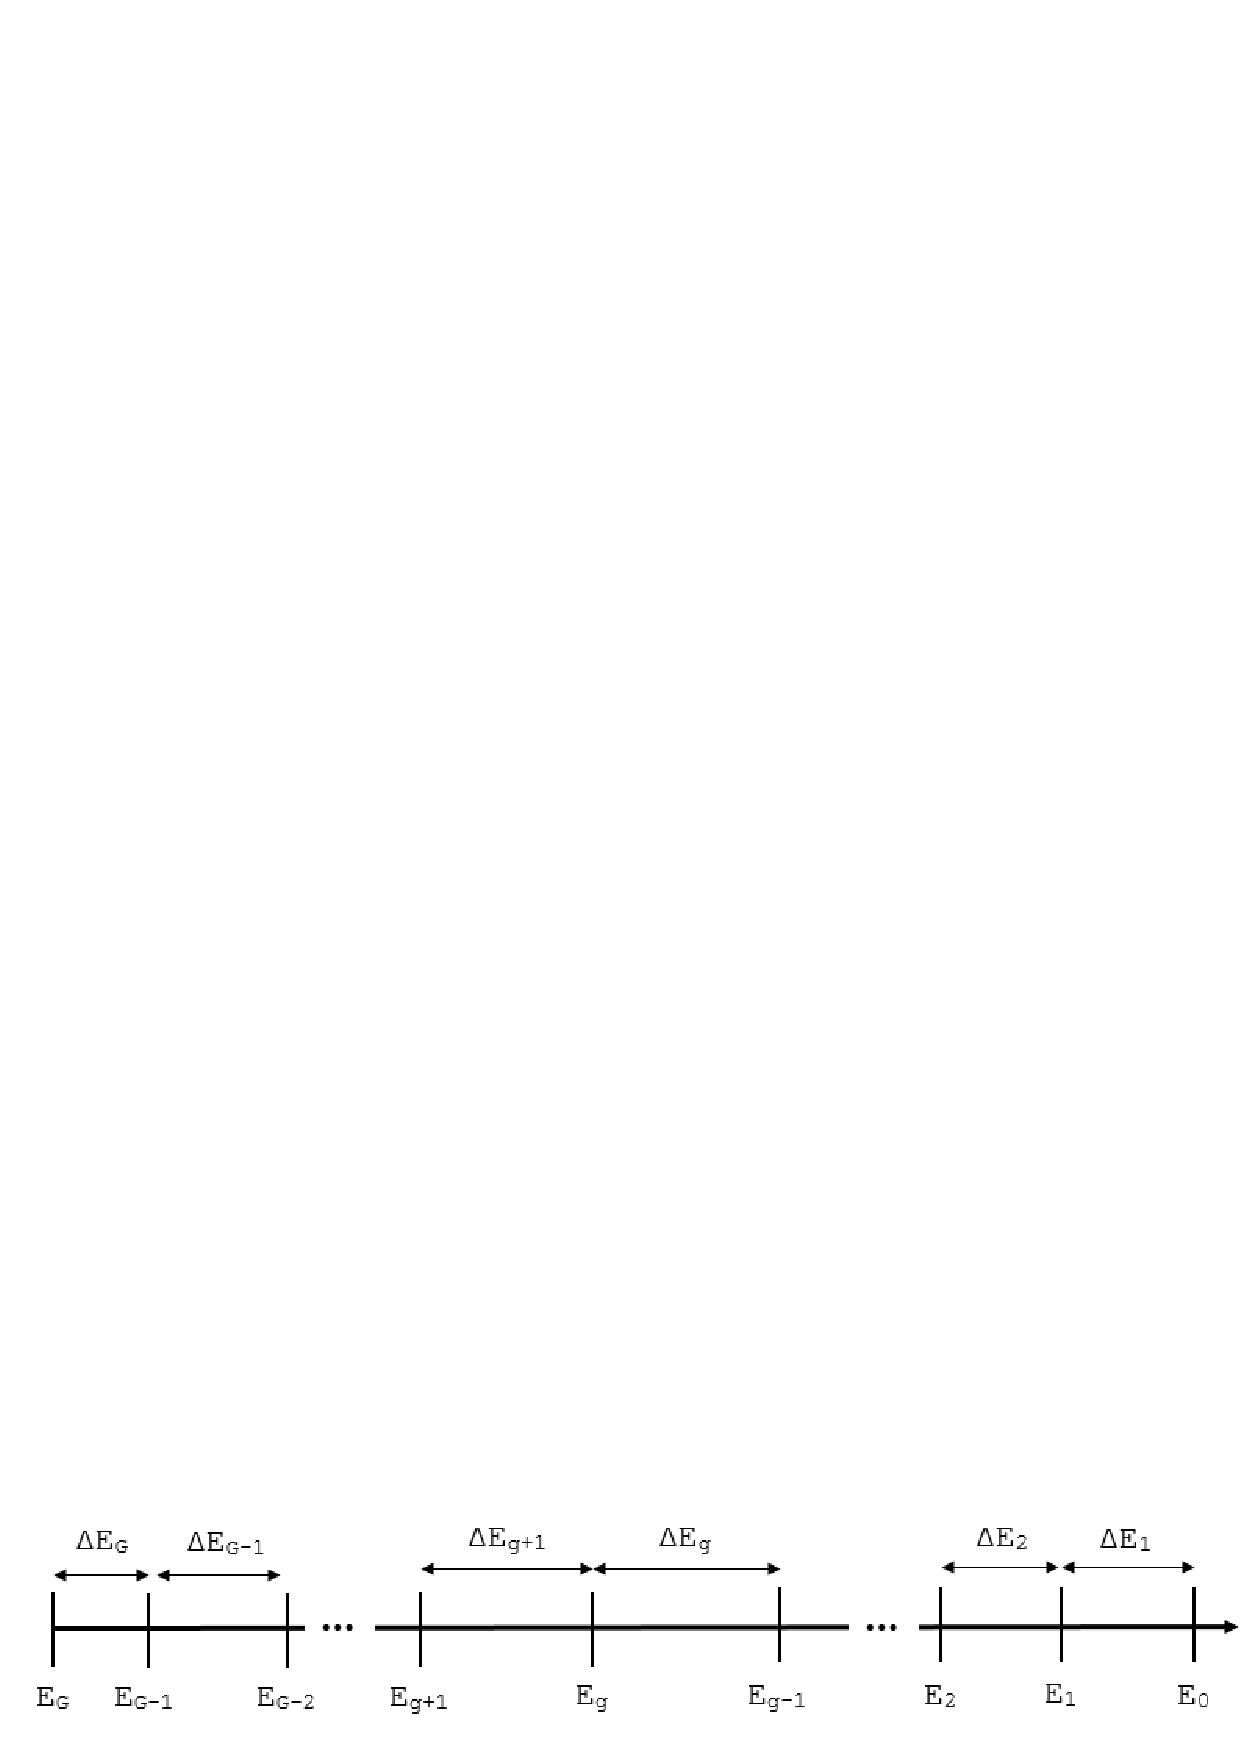
\includegraphics[width=1.00\textwidth]{figures/sec_Sn/MG_Energy_Bands.pdf}
\caption{Interval structure of the multigroup methodology.}
\label{fig::MG_energy_bands}
\end{figure}



\begin{equation}
\label{eq::Sn_transport_operators_MG}
\begin{aligned}
	{\bf L}_g \Psi &= \vec{\Omega} \cdot \vec{\nabla} \Psi (\vec{r}, E, \vec{\Omega},t)+ \sigma_t (\vec{r}, E,t) \Psi (\vec{r}, E, \vec{\Omega},t), \\
	{\bf F}_g \Psi &= \frac{\chi (\vec{r}, E,t)}{4 \pi} \int dE' \nu \sigma_f (\vec{r}, E',t) \int d\Omega' \Psi (\vec{r}, E', \vec{\Omega}',t), \\
	{\bf S}_g \Psi &= \int dE' \int d\Omega' \sigma_s (E' \rightarrow E, \Omega' \rightarrow \Omega) \Psi (\vec{r}, E', \vec{\Omega}'),  \\
	{\bf Q}_g       & = Q_{ext} (\vec{r}, E, \vec{\Omega},t)
\end{aligned}
\end{equation}

\begin{figure}[!hbt]
\centering
	\begin{subfigure}[b]{0.58\textwidth}
		\centering
		\label{subfig::unit_square}
		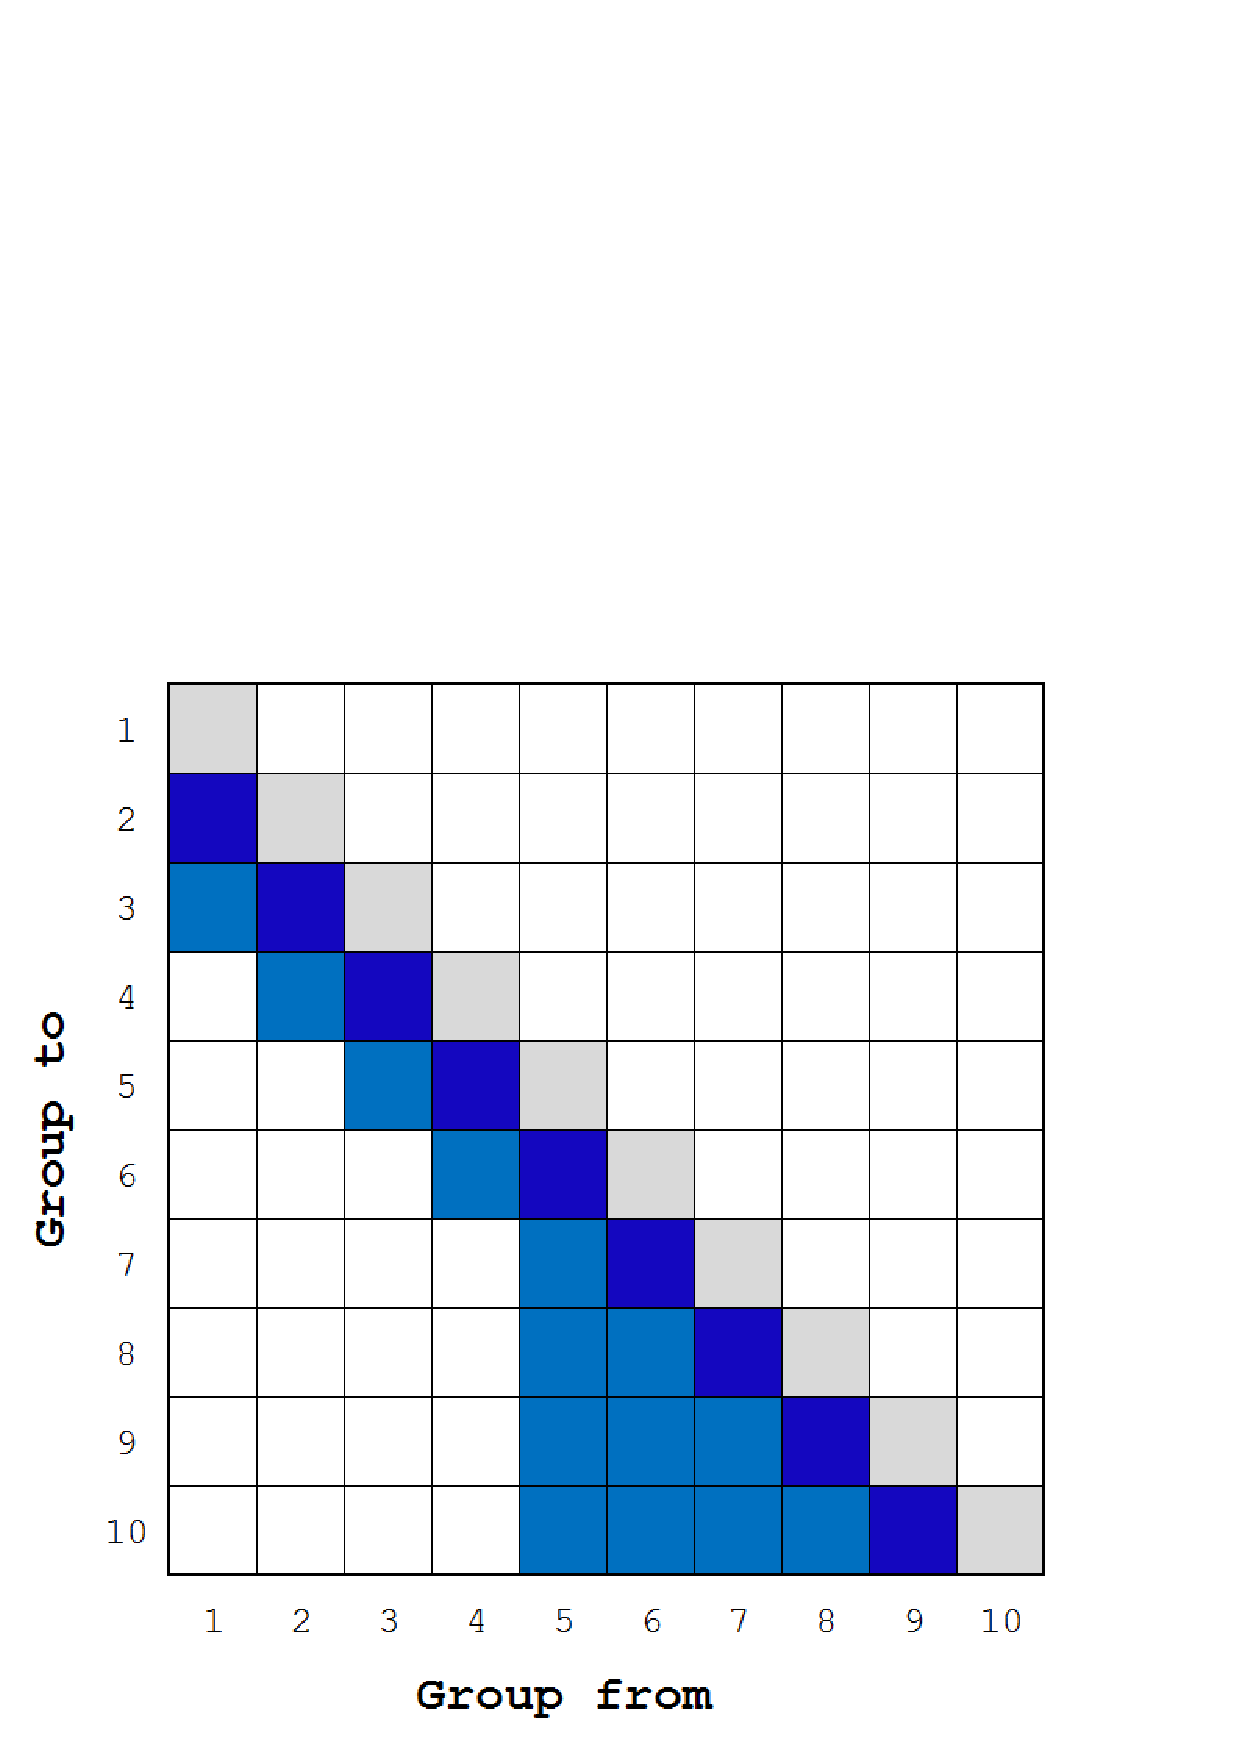
\includegraphics[width=\textwidth]{figures/sec_Sn/scattering_matrix_NO_upscattering.pdf}
		\vspace{4mm}
	\end{subfigure}
	\hfill
	\begin{subfigure}[b]{0.58\textwidth}
		\centering
		\label{subfig::unit_cube}
		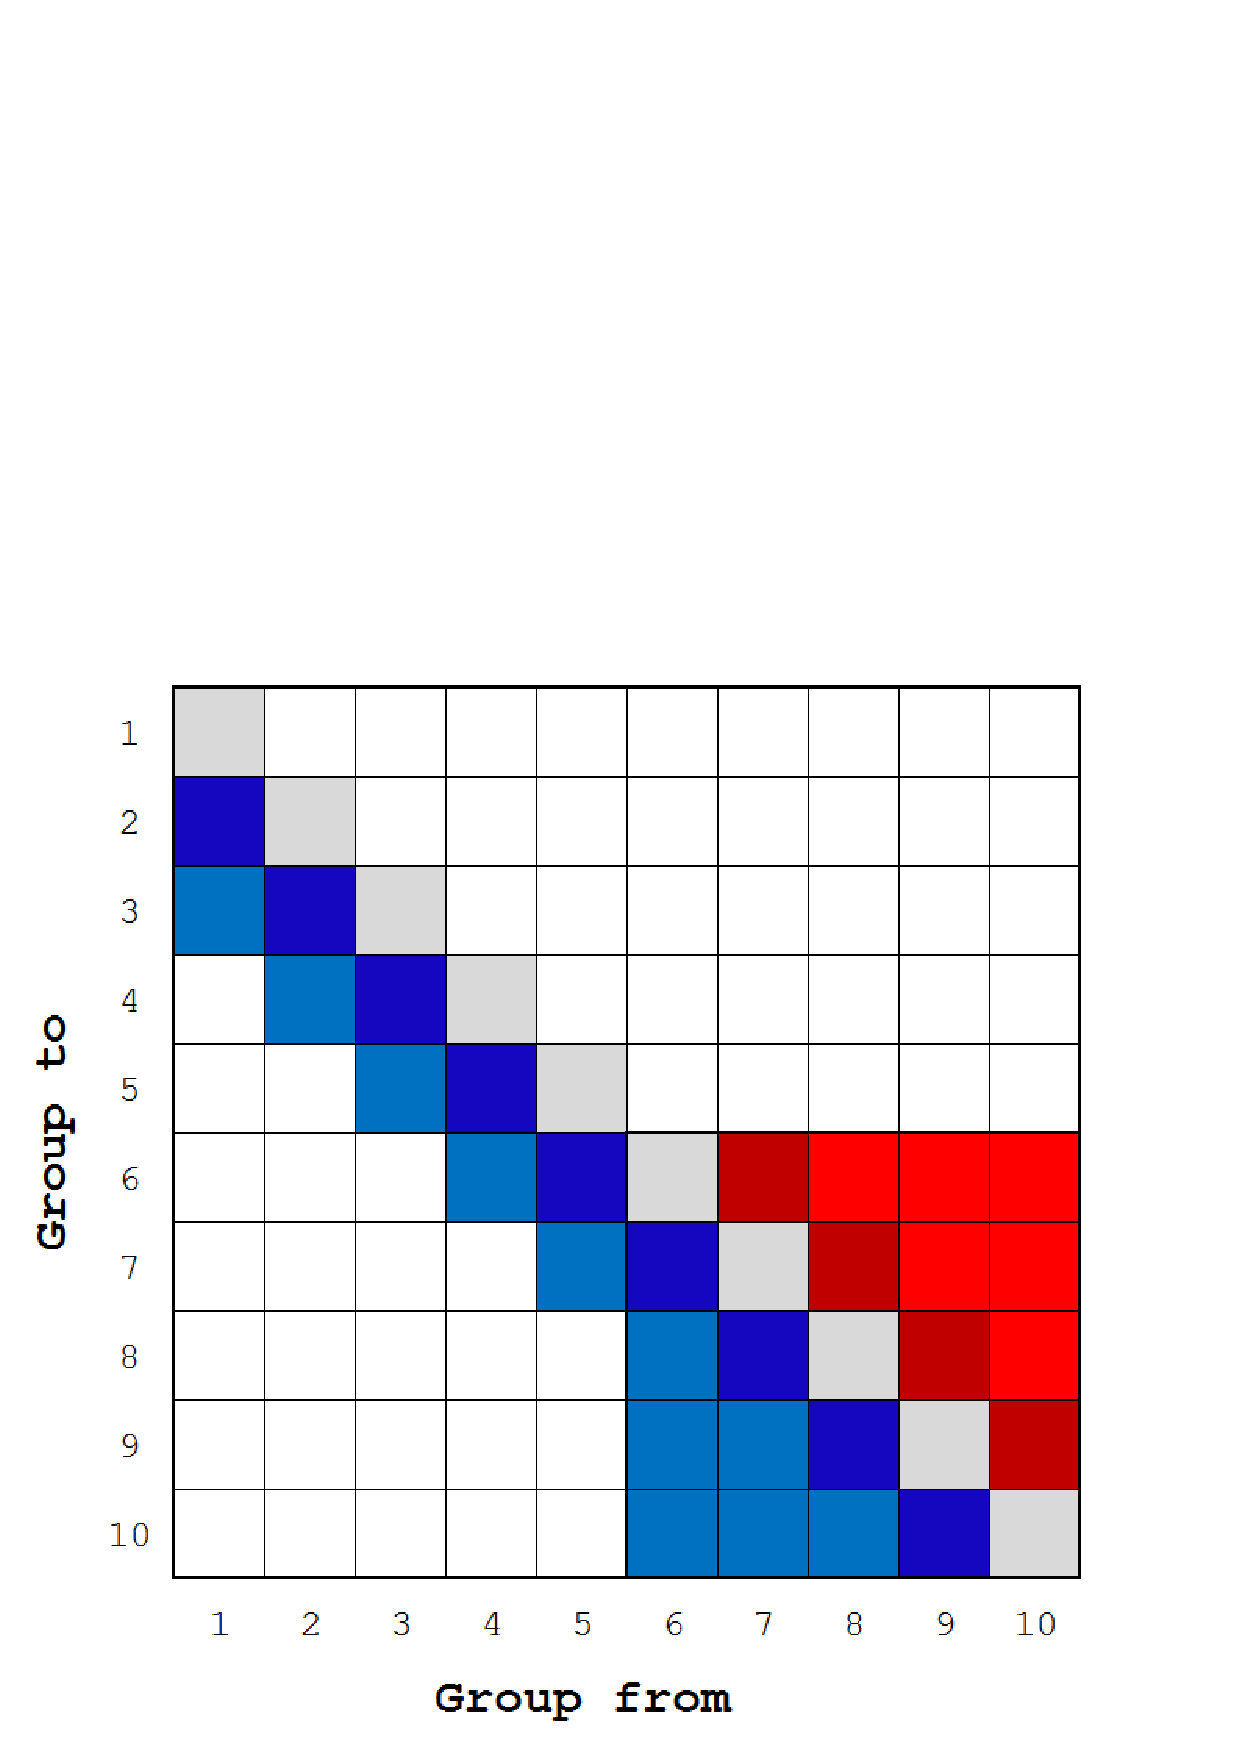
\includegraphics[width=\textwidth]{figures/sec_Sn/scattering_matrix_w_upscattering.pdf}
	\end{subfigure}
\caption{Scattering matrices (top) without and (bottom) with upscattering. The gray corresponds to within-group scattering; the blue corresponds to down-scattering in energy; and the red corresponds to up-scattering in energy.}
\label{fig::BF_scattering_matrix}
\end{figure}

%%%%%%%%%%%%%%%%%%%%%%%%%%%%%%%%%%%%%%%%%%%%%%%%%%%
%%%   Section - Angle Discretization
\section{Angular Discretization}
\label{sec::Sn_Angle}

%%%%%%%%%%%%%%%%%%%%%%%%%%%%%%%%%%%%%%%%%%%%%%%%%%%
%%%   Section - Spatial Discretization
\section{Spatial Discretization}
\label{sec::Sn_Spatial}

Using the energy and angular discretizations presented in Sections \ref{sec::Sn_MG} and \ref{sec::Sn_Angle}, respectively, we write the standard, steady-state, multigroup $S_N$ transport equation for one angular direction, $m$, and one energy group, $g$:

\begin{equation}
\label{eq::Sn_mg_sn_trans_eq}
\begin{aligned}
	 \left( \vec{\Omega}_m \cdot \vec{\nabla}  + \sigma_{t,g} (\vec{r}) \right)  \Psi_{m,g} (\vec{r}) = \sum_{g'=1}^{G} \sum_{p=0}^{N_P} \frac{2p + 1}{4 \pi} \sigma_{s,p}^{g' \rightarrow g}  (\vec{r}) \sum_{n=-p}^{p}  \Phi_{p,n,g'}  (\vec{r})  Y_{p,n} \left(  \vec{\Omega}_m \right)  \\
	+ \frac{\chi_g}{4 \pi} \sum_{g'=1}^{G} \nu \sigma_{f,g'} \Phi_{g'}  (\vec{r})  + Q_{m,g}  (\vec{r}) 
\end{aligned}
\end{equation}

\noindent with the following general, discretized boundary condition:

\begin{equation}
\label{eq::Sn_mg_sn_trans_eq_bc}
\Psi_{m,g} (\vec{r}) = \Psi^{inc}_{m,g} (\vec{r}) + \sum_{g'=1}^{G} \sum_{\vec{\Omega}_{m'} \cdot \vec{n} > 0} \gamma_{g' \rightarrow g}^{m' \rightarrow m} (\vec{r})  \Psi_{m',g'} (\vec{r}) 
\end{equation}

%%%%%%%%%%%%%%%%%%%%%%%%%%%%%%%%%%%%%%%%%%%%%%%%%%%
%%%   SubSection - Mass
\subsection{Elementary Mass Matrices}
\label{sec::Sn_Spatial_Mass}

In the spatially discretized equations presented in Section \ref{sec::Sn_Spatial}, there are several reaction terms that appear with the form: $\Big< \sigma \psi_m, b_m  \Big>_K$ for a given angular direction, $m$, and for a spatial cell, $K$. In FEM analysis these reaction terms are ubiquitously referred to as the mass matrix terms \cite{zeinkiewicz2005finite}. For cell $K$, we define the elementary mass matrix, ${\bf M}$ as

\begin{equation}
\label{eq::Sn_mass_matrix_analytical}
{\bf M}_K =    \int_K {\bf b}_K \, {\bf b}_K^T \, d {\vec{r}} ,
\end{equation}

\noindent where ${\bf b}_K$ corresponds to the set of $N_K$ basis functions that have non-zero measure in cell $K$. Depending on the FEM basis functions utilized, the integrals in Eq. (\ref{eq::Sn_mass_matrix_analytical}) can be directly integrated analytically. However, if in general, the basis functions cannot be analytically integrated on an arbitrary set of cell shapes, then a numerical integration scheme becomes necessary. 

\begin{equation}
\label{eq::Sn_mass_matrix_numerical}
{\bf M}_K =    \sum_{} {\bf b}_K \, {\bf b}_K^T \, d {\vec{r}} ,
\end{equation}


\begin{equation}
\label{eq::Sn_mass_matrix_array}
{\bf M}_K =   \left[
\begin{array} {ccccc}
	\int_K b_1 \, b_1  & \ldots & \int_K b_1 \, b_j  & \ldots & \int_K b_1 \, b_{N_K} \\
	\vdots  &  & \vdots  &  & \vdots \\
	\int_K b_i \, b_1  & \ldots & \int_K b_i \, b_j  & \ldots & \int_K b_i \, b_{N_K} \\
	\vdots  &  & \vdots  &  & \vdots \\
	\int_K b_{N_K} \, b_1  & \ldots & \int_K b_{N_K} \, b_j  & \ldots & \int_K b_{N_K} \, b_{N_K} \\
\end{array}
\right]
\end{equation}


%%%%%%%%%%%%%%%%%%%%%%%%%%%%%%%%%%%%%%%%%%%%%%%%%%%
%%%   SubSection - Streaming
\subsection{Elementary Streaming Matrices}
\label{sec::Sn_Spatial_Streaming}

Next, we will consider the streaming term that has the form: ${\Omega}_m \cdot \Big< \vec{\nabla} \psi_m, b_m  \Big>_K$ for a given angular direction, $m$, and for a spatial cell, $K$. $\vec{\nabla} $ is the gradient operator in physical space and has the form in 1 dimension of 

\begin{equation}
\label{eq::grad_op_1D}
	\vec{\nabla} = \left[ \frac{d}{dx} \right], 
\end{equation}

\noindent in 2 dimensions of

\begin{equation}
\label{eq::grad_op_2D}
	\vec{\nabla} = \left[ \frac{\partial}{\partial x} , \frac{\partial}{\partial y} \right], 
\end{equation}

\noindent and in 3 dimensions of 

\begin{equation}
\label{eq::grad_op_3D}
	\vec{\nabla} = \left[ \frac{\partial}{\partial x} , \frac{\partial}{\partial y} , \frac{\partial}{\partial z} \right].
\end{equation}

\noindent Since

\begin{equation}
\label{eq::Sn_streaming_matrix_analytical}
\vec{{\bf G}}_K =    \int_K \vec{\nabla} {\bf b}_K \, {\bf b}_K^T \, d {\vec{r}} ,
\end{equation}

\begin{equation}
\label{eq::Sn_streaming_matrix_array}
\vec{{\bf G}}_K =   \left[
\begin{array} {ccccc}
	\int_K \vec{\nabla}b_1 \, b_1  & \ldots & \int_K \vec{\nabla}b_1 \, b_j  & \ldots & \int_K \vec{\nabla}b_1 \, b_{N_K} \\
	\vdots  &  & \vdots  &  & \vdots \\
	\int_K \vec{\nabla} b_i \, b_1  & \ldots & \int_K \vec{\nabla}b_i \, b_j  & \ldots & \int_K \vec{\nabla}b_i \, b_{N_K} \\
	\vdots  &  & \vdots  &  & \vdots \\
	\int_K \vec{\nabla} b_{N_K} \, b_1  & \ldots & \int_K \vec{\nabla} b_{N_K} \, b_j  & \ldots & \int_K \vec{\nabla} b_{N_K} \, b_{N_K} \\
\end{array}
\right]
\end{equation}

%%%%%%%%%%%%%%%%%%%%%%%%%%%%%%%%%%%%%%%%%%%%%%%%%%%
%%%   SubSection - Surface
\subsection{Elementary Surface Matrices}
\label{sec::Sn_Spatial_Surface}


%%%%%%%%%%%%%%%%%%%%%%%%%%%%%%%%%%%%%%%%%%%%%%%%%%%
%%%   Section - Conclusions
\section{Conclusions}
\label{sec::Sn_Conclusions}

In this chapter